\chapter{Virtualization and Cloud Computing}
\label{chapter:cloudcomputing}

%General about the shift that has been happening towards virtualized and software applications



\textcolor{red}{More prepping on virtualization}

Virtualization is a technology that allows creating valuable IT services using resources that are traditionally bound to hardware. Virtualization allows hardware operators to use the physical machine's full capacity by distributing the computing power to multiple users or environments. \cite{RedHat} In the context of telco, virtualization the main objective is to replace the costly dedicated hardware implementing several centralized control plane functions and other services with distributed solutions that may be allocated on-demand over a pool of dependable, dynamically contracted computing and networking resources that are easy to manage. \cite{Bosch2011} Virtualization brings down the expenses arising from acquiring, updating, and managing the hardware.

\subsection{Hardware support}

\section{Virtualization types}
\textcolor{red}{Introduce Kata and other similar virtualization types here}
\textcolor{red}{Describe each virtualization type more}

A traditional server has applications running directly on the host operating system (OS). The solution limits overhead from extra layers such as hypervisor or virtual machine (VM), but compromises the usage of resource efficiency, security and limits compatibility. Two virtualization technologies, hypervisor-based virtualization and operating system -level virtualization, have been introduced to improve these features. Figure \ref{fig:VirtualizationTypes} describes the stack of these two virtualization types and a traditional physical server.

\begin{figure}[ht]
  \begin{center}
    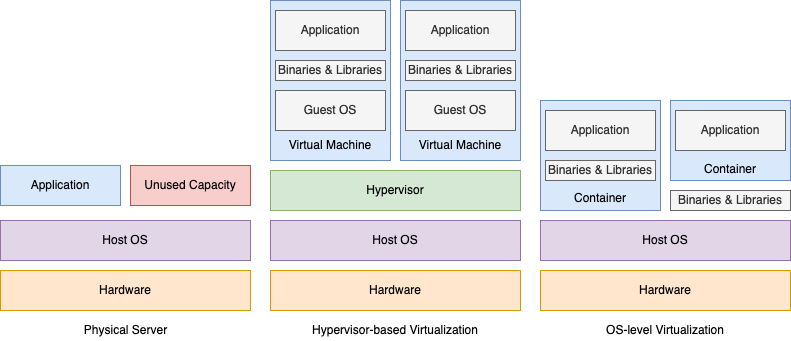
\includegraphics[width=13.5cm]{images/VirtualizationTypes.png}
    \caption{Physical server and two types of virtualization}
    \label{fig:VirtualizationTypes}
  \end{center}
\end{figure}

First of the virtualization technologies, hypervisor-based virtualization adds a hypervisor on top of the host OS and each application instance running is wrapped inside a VM with a dedicated guest OS, binaries, and libraries. This approach is secure and compatible with various host operating systems and processor architectures via hardware emulation. However, the added layers increase the performance overhead significantly. Resources of the server are wasted, especially when multiple VMs are hosted on the same server. In contrast, OS-level virtualization with containers replace the bulky OS with minimal image, such as Alpine. Containers are isolated areas in the host operating system and they do not include an additional guest operating system inside them. Instead, to enable operating system-like functionality, they share parts of the host kernel as well as the host’s libraries and binaries where appropriate. These containers can also include application specific binaries and libraries. \cite{Toimela2017}

\section{Cloud computing}

Data centers, with the help of hardware virtualization, offer on-demand availability of computer resources such as computing power or data storage. This pay-per-use offering is described as cloud computing. It has been a vital enabler in the field of Information Technologies allowing the success of cloud applications such as Google Docs, Slack, and Dropbox. The ubiquitous and connected computing provided allows higher usage of resources and access from anywhere via internet, thus improving performance, reducing costs, and allowing easy access to hosted applications. Public cloud services end-user spending worldwide has been growing steadily and is expected to grow 40\% from 2020's 219 billion euro to 307 billion euro only in two years \cite{PublicCloudStatista}.

The general idea behind cloud computing technology dates back to the emerge of grid computing in early 1990s as an idea for making computing power as easy to access as an electric power grid. This cloud model promotes availability and is composed of five essential characteristics. These characteristics are on-demand self-service, ubiquitous network access through Internet-enabled devices, location independent resource pooling, rapid elasticity, and pay per use. \cite{Xing2012}

A cloud is a pool of virtualized resources across the internet, that follows pay-per-use model and can be dynamically reconfigured to satisfy the user requests by provisioning virtual machines. Cloud computing is a service model for IT provisioning, often based on virtualization and distributed computing technologies \cite{Lombardi2011}. Cloud computing offers four different service models: public, private, hybrid, and community clouds. Cloud is typically a centralized server, such as, Microsoft Azure or Red Hat OpenShift. These cloud platforms provide users with scalable resources, high availability and fast connections. Cloud platforms can be public, such as the before-mentioned ones, or a private cloud serving only selected customers. Private clouds are usually deployed on-premises within a corporate firewall by businesses with requirements for additional control and privacy over the network. Hybrid cloud is a combination of both, made up of on-premises infrastructure, private cloud services, and a public cloud. The hybrid approach brings enterprise with agility to use the best suitable solution for each occasions. \cite{NetApp} Community cloud is a resource pool that consists of an aggregation of several providers, which can be shared by a certain group of users. \cite{Taleb2017}\cite{MicrosoftAzure}\cite{Xing2012}

% Emerge of various applications with different requirements
% Optimize latency and throughput in network
% Intro to Edge



\section{Edge Computing}
\textcolor{red}{More prepping on edge computing}

Telecommunications computing ... The computing locates in various data centers as described in Figure \ref{fig:AirFrame}. Central data centers are built to massive warehouses that take advantage of centralized maintenance and 

Telco environment
Central data center vs edge cloud in general
    - Efficient capacity vs low latency \& efficient transport


\begin{figure}[ht]
  \begin{center}
    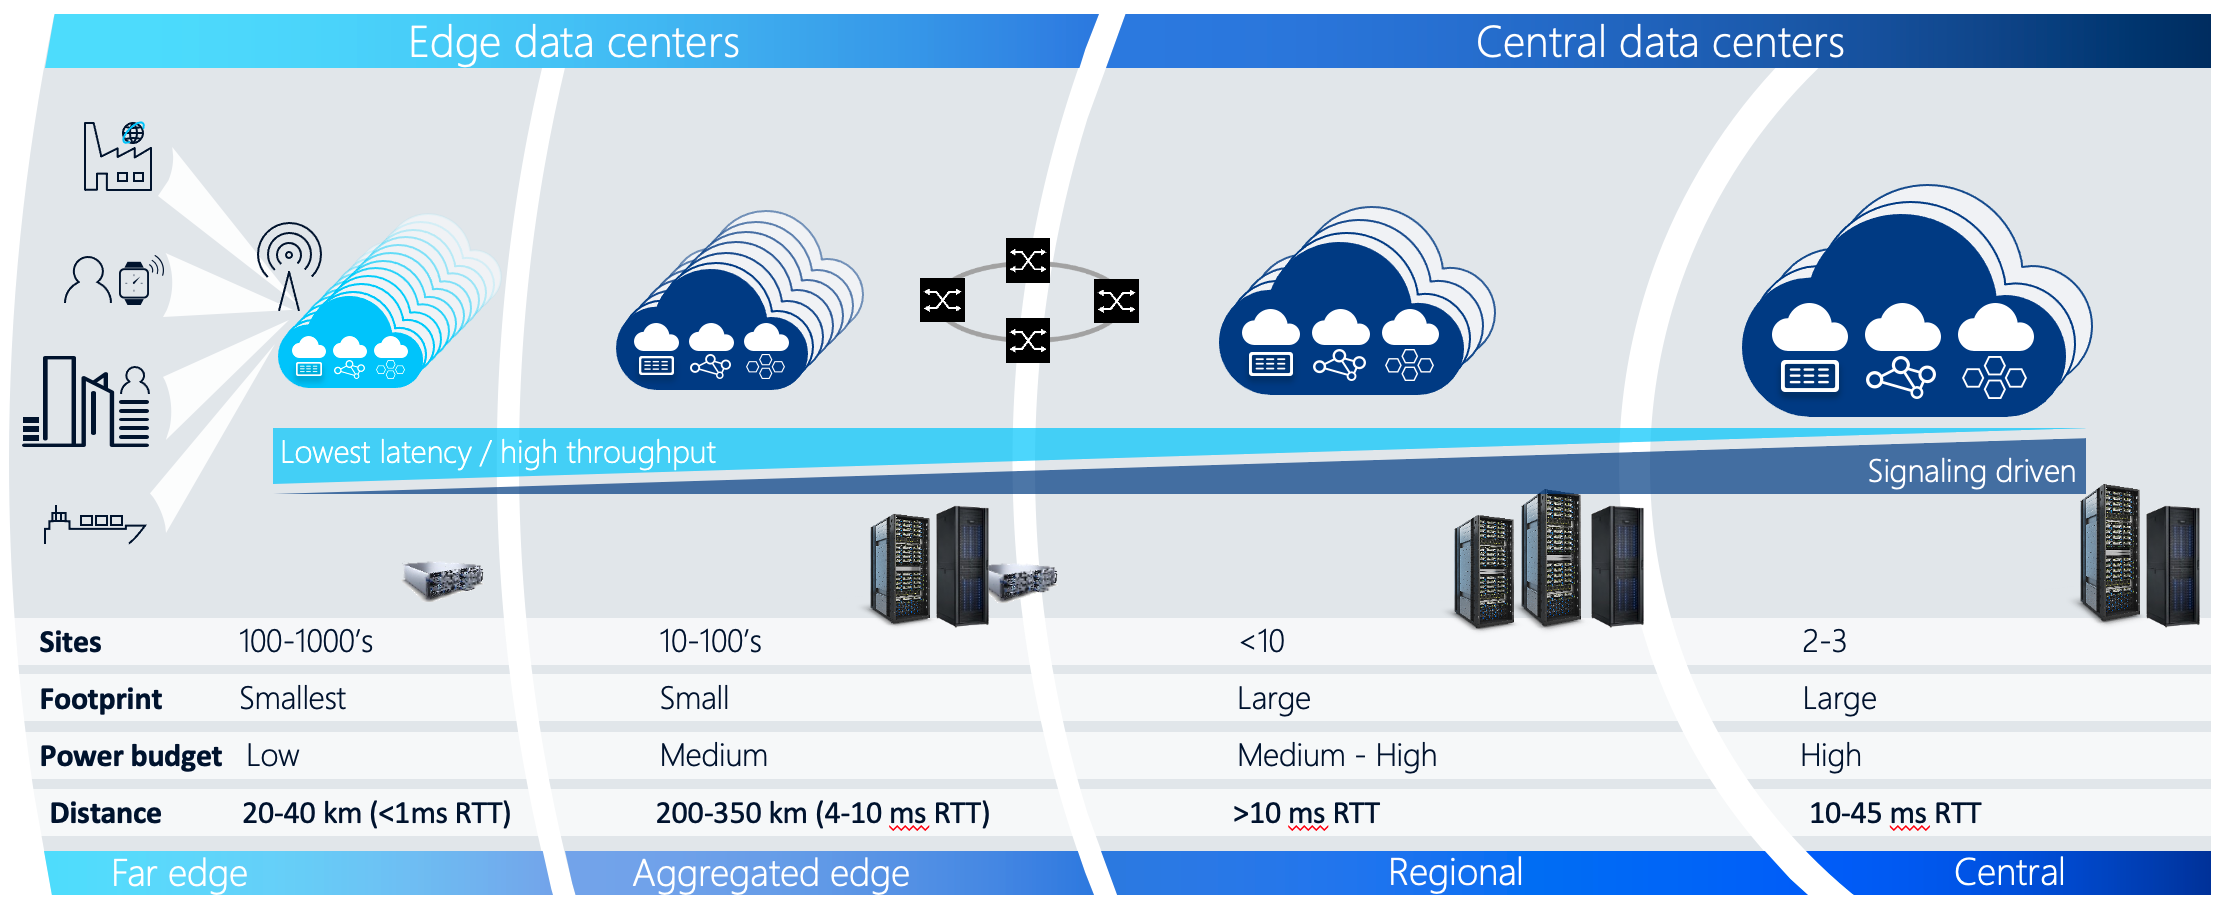
\includegraphics[width=13.5cm]{images/AirFrame.png}
    \caption{Far edge comparison to central data center \cite{AirFrameOpenEdgeServer}}
    \label{fig:AirFrame}
  \end{center}
\end{figure}

\section{Multi-access Edge Computing}

Multi-access Edge Computing (MEC) is an emergent architecture where  cloud computing services are extended to the edge of networks leveraging mobile base Radio Access Network (RAN) improving the delivery of content and applications to end user. As a promising edge technology, it can be applied to mobile, wireless, and wireline scenarios, using software and hardware platforms, located at the network edge in the vicinity of end-users. MEC provides seamless integration of multiple application service providers and vendors toward mobile subscribers, enterprises, and other vertical segments. It is an important component in the 5G architecture which supports variety of innovative applications and services where ultra-low latency is required. \cite{Abbas2018}

MEC improves network efficiency by processing and storing data on the mobile network cell instead of hauling it completely back to regional or central data centers for processing. The data can be processed partially or completely on the MEC node. For example, large public venues, such as stadiums or arenas, are good candidates for MEC, especially where localized venue services are important. In this use case, video created at a sports event or concert is served to on-site consumers from a MEC server, running appropriate applications located on the stadium premises. This video traffic is locally stored, processed and delivered directly to users at the event and does not require backhaul to a centralized core network and to then be returned to the user at the venue. The local processing of data reduces perceived latency on end-user and limits stress on the backhaul network. \cite{Brown2016}

MEC covers two edge entities: aggregated edge and far edge. Aggregated edge locates usually at most 200 to 350 kilometers away from the end user and guarantees 4 to 10 millisecond round trip time (RTT). The RTT is low in comparison to central data center latency, however it is not low enough for mission-critical applications requiring less than 1 ms latency. For example, self-driving cars and factory robots might require ultra-low latency reply from the applications.

\subsection{Far Edge Cloud}

Far edge cloud locates at most 20 to 40 kilometers away from the end user, and thus is able to offer sub one millisecond RTT, as service level agreement of the 5G network \cite{Parvez2018}. The ultra-low latency is critical for applications requiring instant reply from the server. Offloading tasks, computing, and storage to nearby cloud allows thin clients, such as cellphones or dashboards, with limited resources to support applications with resource heavy requirements, such as applying machine learning models to obtained video feed in real-time. Far edge cloud setup is minimal in size, footprint, and power budget. It is flexible to install as it can be located in an office or apartment building with no requirement for extensive server chassis. \cite{AirFrameOpenEdgeServer}

Far edge cloud units are highly localized. A network might consist of hundreds or thousands of these units. The data processed does not always travel further away from the end-user enhancing the security and integrity of the data. The localized data schemes help also service providers, as they are not obliged to apply multiple data protection laws, GDPR for example, at the same time. FEC units also handle sensitive, user-related data. Thus, it is crucial to secure the infrastructure from external threats and internal attacks, such as third-party applications hosted on the infrastructure.

\subsection{Applications}
\label{subs:applications}

MEC architecture unlocks potential of new applications, and thus is a new revenue stream for mobile network operators. Some recognized applications harnessing the use of MEC include augmented reality (AR), video analytics, and connected vehicles.

AR enables real environment user experience by combining real and virtual objects existing simultaneously. Recent AR applications have become adaptive in sound and visual components, such as news, TV programs, sports, object recognition, and games. AR applications often demand high computational resources, low latency for reasonable quality-of-experience, and high bandwidth. MEC can empower AR applications by maximizing throughput by offering computational resources nearby the end-user withing low-latency and high throughput channel instead of relying on the core-network. \cite{Abbas2018}

Surveillance cameras traditionally have been streaming data back to the server, which decides how to perform data analysis. Due to the growing number of these cameras, it adds an enormous stress to the network with the constant data streams. In this example, MEC will be beneficial by implementing intelligence to the device by transmitting data only when motion is detected. Also, it can help public safety with detection of traffic jams, accidents or forest fires.

Connected vehicles are facilitated with cellular connection allowing them to communicate with other users on the road. MEC based road communication system could allow two-way communication between vehicles via road side units. For example, one vehicle could warn another vehicles about upcoming road jam or approaching pedestrians. The road side unit could also warn passing cars about dangerous conditions based on the sensors equipped in it. \cite{Abbas2018}

\section{Security concerns}

Integrity and confidentiality concerns are still problems in cloud computing that call for effective and efficient solutions. Cloud nodes are inherently more vulnerable to cyber-attacks and breaches than traditional solutions, given their size and the underlying complexity of services bringing unprecedented exposure to third parties of services and interfaces. \cite{Lombardi2011}

Cloud and Edge Computing security cover the same threats as core computing. However, these platforms are generally not offering the same security-rich features and security policies and procedures. Edge Computing is typically more vulnerable to local introspection attacks. \cite{EdgeComputing5G} 

Cloud and edge computing allow service providers and MNOs for more flexible and cost-efficient service deployment due to shared and decentralized infrastructure. Especially MNOs seek to unlock extra revenue streams by offering their infrastructure to host applications such as mentioned in Chapter \ref{subs:applications}. In order to mitigate costs from the application, it is resource-efficient to run multiple instances or applications from various parties on a single server. This approach applies to companies who own dedicated servers or cloud computing providers with various data center options. These multi-tenant environments may host applications also from untrusted parties. Regardless of the isolation offered by Docker with cgroups and namespaces, the containers still share the same kernel. This architectural decision might expose applications, as it was noticed in 2019 \cite{CVE-2020-14386}\cite{CVE-2019-5736} when attackers could elevate their access to host root. The escaping of container and horizontal traversal via shared kernel creates a security thread of application data integrity. The virtualization technique domain is buoyant with many competing emerging technologies for hardening containers and VMs, solving the equation of isolation versus overhead. This thesis researches and evaluates Kata Containers to adding an extra layer of security to avoid the container escapes on host compromise on a shared platform with minimal overhead. \cite{EdgeComputing5G}

%You can translate your latex file to rtf with the \texttt{latex2rtf} command in the
%kosh.aalto.fi shell server. Then, the line breaks
%will not be problems for the proofreader of Word.

%Note also that if you have a section or a subsection, you have to have
%at least two of them, or otherwise the section or subsection title is
%unnecessary. Same with the paragraphs: you should not have sections
%with only one paragraph, and single sentence paragraph.

%Aalto library has a comprehensive citation guide ~\cite{bibinstructions}.


% Comment: If your sentence ends in a capital letter write \@ before the period

% If you do need a normal space after a period (instead of
% the longer sentence separator), use \  (backslash and space) after the
% period. Like so: a.\ first item, b.\ second item.